\subsection{iSAM2}
\subsubsection{Introduction and Motivation}
iSAM2 was developed to overcome the practical limitations of iSAM. The core optimization method in iSAM (nonlinear least squares solved through incremental QR factorization) is sound and provides accurate solutions. The bottlenecks arise not from the underlying algorithms, but from the static data structure used to maintain the problem. In iSAM the system is stored as a single global square root information matrix $R$. While this representation is compact and efficient for batch updates, it leads to several issues during incremental operation.
\\ \\
First, the $R$ matrix is ``global''. Adding new factors or loop closures often changes many rows and columns, which requires expensive refactorization. This causes latency spikes, especially when loop closures occur and large parts of the trajectory suddenly become coupled. Second, relinearization in iSAM is also global. To maintain accuracy, the system periodically refreshes Jacobians for all factors, which forces full reconstruction of the $R$ matrix. Third, variable reordering to reduce fill in and keep $R$ sparse is again an all or nothing operation, with cost proportional to the entire problem size. Together, these properties mean that iSAM, while efficient between updates, still suffers from periodic heavy computation that disrupts real time performance.
\\ \\
iSAM2 addresses these limitations by introducing a new data structure, the ``Bayes tree''. Instead of representing the system as a static $R$ matrix, iSAM2 leverages the factor graph formulation of SLAM, applies variable elimination, and interprets the resulting structure as a chordal Bayes net. This Bayes net can then be compactly represented as a Bayes tree, which retains all probabilistic information while enabling local updates. With the Bayes tree, adding new measurements or relinearizing states only modifies the affected cliques in the tree, leaving the rest untouched. This local property eliminates the global refactorization bottlenecks of iSAM, smooths out computation over time, and makes the algorithm scalable to large and long term mapping problems. \cite{iSAM2_paper,Bayes_tree_for_SLAM_paper}



\subsubsection{Factor Graphs}
A factor graph is a bipartite graph that connects variable nodes (poses and landmarks) to factor nodes (priors, motion, and measurements). It encodes the same estimation problem as in iSAM, but makes sparsity and locality explicit because each factor touches only a few variables.
\\ \\
Let the variables be robot poses $x_1,\dots,x_M$ and landmarks $l_1,\dots,l_N$, and let $\Theta=\{x_1,\dots,x_M,l_1,\dots,l_N\}$. According to the iSAM2 papers \cite{iSAM2_paper,Bayes_tree_for_SLAM_paper} the posterior factorizes as
\[
    f(\Theta) = \prod_{i} f_i(\Theta_i),
\]
Here, each factor $f_i$ depends only on its adjacent variables $\Theta_i$. How each factor is modeled depends on the situation. Because odometry and measurements are uncertain in the real world, factors should be represented with a probabilistic model. One of the easiest probabilistic models is Gaussian, which is easy to model and will work well later when working in Mahalanobis form to optimize the problem and solve it in simple manner (See Figure \ref{fig:mahalanobis-distance} for Mahalanobis form). Factor functions can therefore be modeled as follows:
\[
    \text{Prior:}\quad f_p(x_0)\ \propto\ \exp\!\Big(-\tfrac{1}{2}\|\mu_0 - x_0\|_{P_0}^2\Big),
\]
\[
    \text{Odometry:}\quad f_i(x_{i-1},x_i)\ \propto\ \exp\!\Big(-\tfrac{1}{2}\|f_i(x_{i-1},u_i) - x_i\|_{Q_i}^2\Big),
\]
\[
    \text{Measurement:}\quad f_k(x_{i_k},l_{j_k})\ \propto\ \exp\!\Big(-\tfrac{1}{2}\|h_k(x_{i_k},l_{j_k}) - z_k\|_{R_k}^2\Big).
\]
This is in a way very similar to how iSAM models the system, however here in iSAM2, the system is represented as factor graphs. This graph view exposes conditional independence directly in the topology. Each factor only connects nearby variables in time or space, which later yields a sparse linear system.
\\ \\
\begin{figure}[H]
    \centering
    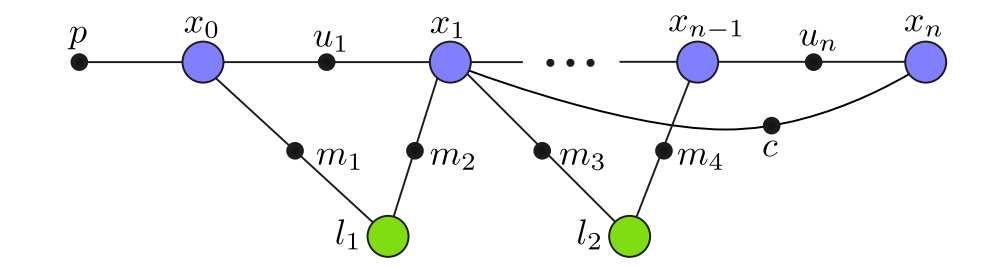
\includegraphics[width=0.98\linewidth]{Pictures/Optimizers/iSAM2/Factor_graph.png}
    \caption{Picture from iSAM2 paper \cite{iSAM2_paper} describes factor graph formulation of the SLAM problem. Variable nodes (large circles) are poses $x_0,\dots,x_n$ and landmarks $l_1,l_2$. Factor nodes (small solid circles) represent a prior $p$, odometry $u_i$, landmark measurements $m_i$, and a loop closure constraint $c$. This approach can represent any cost function, including factors that connect more than two variables.}
    \label{fig:optimizer-iSAM2-factor-graph}
\end{figure}
\noindent
This example shows how local connectivity induces sparsity. This will be useful when solving the optimization problem later down bellow. Each factor touches only its adjacent variables, so after linearization (to compute a local optimum) the Jacobian rows have nonzeros only in those columns. The resulting matrix is sparse, which helps the optimizer.



\subsubsection{From Factor Graphs to the SLAM Optimization Problem}
Here SLAM is represented with a factor graph $G=(\mathcal{F},\Theta,\mathcal{E})$. There are two node types, factor nodes $f_i\in\mathcal{F}$ that encode pieces of information (prior, odometry, measurements, loop closures), and variable nodes $\theta_j\in\Theta$ that hold unknowns (poses, landmarks, calibration). An edge $e_{ij}\in\mathcal{E}$ is drawn only when factor $f_i$ depends on variable $\theta_j$. This wiring is important, missing edges mean independence, and the pattern of edges controls which variables interact in the estimation problem.
\\ \\
The graph specifies how a global objective splits into simple parts:
\[
    f(\Theta)\;=\;\prod_i f_i(\Theta_i),
\]
Here $\Theta_i$ collects only the variables that touch factor $f_i$. In the SLAM setting, a prior $p$ anchors the first pose, odometry factors $u$ relate consecutive poses, landmark factors $m$ couple a pose with a landmark, and loop closure factors $c$ link poses that see the same place again (see Picture \ref{fig:optimizer-iSAM2-factor-graph}). The same framework can also handle factors that involve three or more variables, for example a factor that ties a pose to a landmark and a camera intrinsics block (calibration), or ``separator'' variables shared in cooperative mapping. The key point is that the graph can host any cost term as long as it states which variables it touches.
\\ \\
Under Gaussian measurement models as defined in the previous subsection, each factor has the form:
\[
    f_i(\Theta_i)\ \propto\ \exp\!\Big(-\tfrac12\,\|\,h_i(\Theta_i)-z_i\,\|^2_{\Sigma_i}\Big),
\]
This Gaussian form will simplify calculations as Gaussian is nice to work with. Here $h_i(\cdot)$ predicts what the sensor should see from the current variables $\Theta_i$, $z_i$ is the actual measurement, and $\Sigma_i$ is the measurement covariance. The notation $\|e\|^2_{\Sigma}\triangleq e^\top \Sigma^{-1} e$ is the squared Mahalanobis distance, which measures error in ``units of its noise'' (directions with low variance are penalized more). (See Picture \ref{fig:mahalanobis-distance})
\\ \\
To combine all information, simply multiply the factor likelihoods. Products are awkward to optimize, instead take a negative logarithm to turn the product into a sum. Terms that do not depend on $\Theta$ drop out, and each Gaussian factor becomes a squared Mahalanobis residual weighted by its covariance. The result is one scalar objective that collects the prior, all odometry factors, all landmark measurements, and any loop closures. Small covariances make a factor count more, large covariances count less. In short, multiply the factors and take the negative log to get a single sum of squared errors. This can be write in compact form as:
\[
    \Theta^\star \;=\;\arg\min_{\Theta}\ \frac12\sum_i \|\,h_i(\Theta_i)-z_i\,\|^2_{\Sigma_i}
\]
Here $Theta$ collects all unknowns, such as poses, landmarks, and other parameters. Each factor $h_i$ depends only on a small subset $\Theta_i$, so each residual couples only those variables. After linearization this gives a sparse system, because most variables do not appear together in any single residual.
\\ \\
This is our MAP function in nonlinear form.
\\ \\
This nonlinear cost is not solved in one shot because the measurement transform $h_i(\cdot)$ is nonlinear (because of angles, ranges, bearing-only sensors, etc...). As in the iSAM system, linearize around the current estimate and solve iteratively. Choose a current estimate $\Theta^0$ and look for a small update $\Delta\theta$ that improves the fit. For each factor take a 1st-order Taylor expansion around $\Theta^0$, which turns that factor into a simple linear residual in the increment $\Delta\theta$ that touches only its adjacent variables. After whitening by $\Sigma_i^{-1/2}$, stack all linearized factors into one sparse least-squares problem:
\begin{equation}
    \begin{aligned}
        \Delta\Theta^\star = \arg\min_{\Delta\Theta} \left( -log\left(f(\Delta\Theta)\right) \right) = \Delta\theta^\star = \arg\min_{\Delta\theta}\ \|A\,\Delta\theta - b\|^2
    \end{aligned}
    \label{eq:optimizer-iSAM2-least-square}
\end{equation}
Here $A\in\mathbb{R}^{m\times n}$ is the measurement Jacobian (one row block per factor), $b$ stacks the whitened prediction errors, and $\Delta\theta$ is the $n$-dimensional increment. The sparsity pattern of $A$ is dictated by the factor graph, a row has nonzeros only in the columns of the variables that appear in that factor.
\\ \\
Here the linear least squares problem is solved in a numerically stable manner. One route is the normal equations $A^\top A\,\Delta\theta = A^\top b$ and a Cholesky factorization $A^\top A = R^\top R$ followed by forward and back substitution to recover $\Delta\theta$. Another route is QR factorization on $A$, which yields an upper triangular system $R\,\Delta\theta = d$ that can be solved by back substitution. Both routes are standard, in practice QR factorization methods are preferred for stability.
\\ \\
After solving for $\Delta\theta$, update the state $\theta \leftarrow \theta + \Delta\theta$ and repeat, linearize, solve, update. This is Gauss-Newton. If the problem is difficult (poor linearization, strong nonlinearity), add Levenberg-Marquardt damping and instead solve $(A^\top A + \lambda I)\Delta\theta = A^\top b$, which blends Gauss-Newton with a trust-region step to keep updates safe. Stop when $\Delta\theta$ is small or the cost no longer decreases.
\\ \\
This is the same least squares core as in iSAM. The difference is the data structure. iSAM works with the Jacobian $A$ and its triangular factor $R$. iSAM2 keeps the factor graph as the main object, which carries the same information as $A$ from iSAM but in a graph form. Eliminate variables to get a Bayes net and store it as a Bayes tree. This lets iSAM2 update only the cliques touched by new factors instead of refactoring everything. The next subsection shows how this is done.



\subsubsection{From Factor Graphs to Bayes Networks}
\begin{figure}[H]
    \centering
    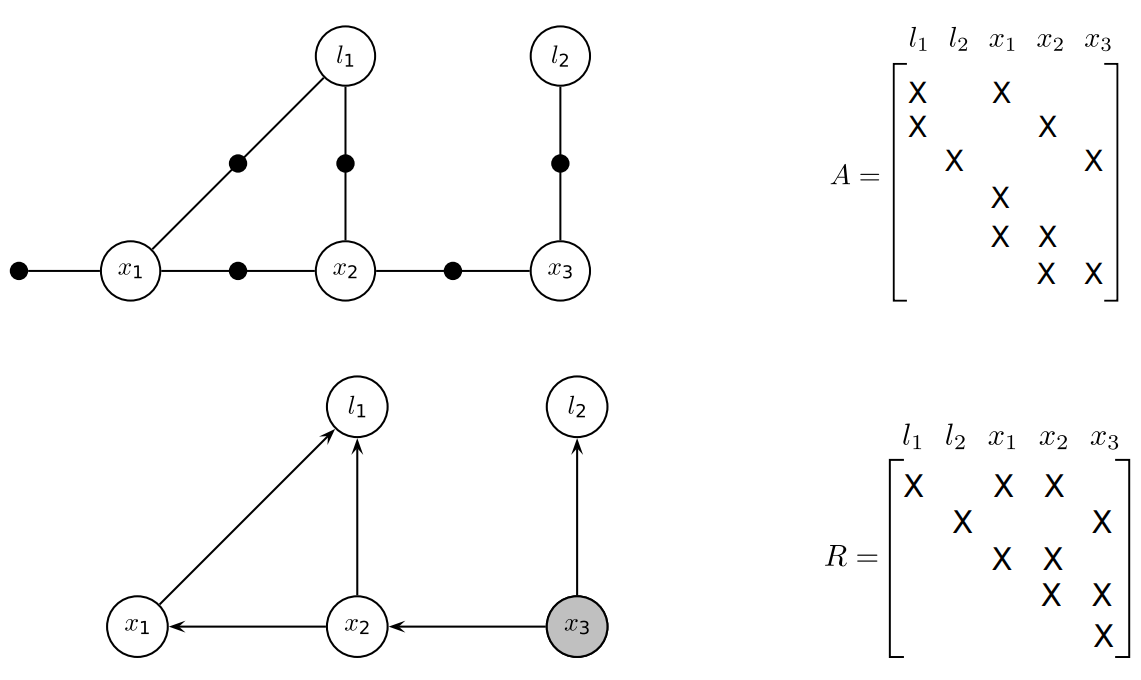
\includegraphics[width=0.98\linewidth]{Pictures/Optimizers/iSAM2/Factor_graph_to_Bayes_network.png}
    \caption{Picture from iSAM2 paper \cite{iSAM2_paper}. (Top) factor graph and associated Jacobian $A$ for a small SLAM example with poses $x_1,x_2,x_3$, landmarks $l_1,l_2$, and a prior on $x_1$ (Bottom) the chordal Bayes net and the square root factor $R$ obtained by eliminating in the order $l_1,l_2,x_1,x_2,x_3$. The last eliminated variable (the root) is shaded. \cite{iSAM2_paper}}
    \label{fig:optimizer-iSAM2-factor-graph-to-bayes-netwrok}
\end{figure}
\noindent
Starting from the least squares form in \eqref{eq:optimizer-iSAM2-least-square}, the whitened measurement matrix $A$ is factored as in iSAM. An elimination order is chosen, (for the example in Picture \ref{fig:optimizer-iSAM2-factor-graph-to-bayes-netwrok} it is $l_1,l_2,x_1,x_2,x_3$), and sparse QR with Givens rotations \eqref{eq:optimizer-iSAM-givens-rotation} is applied. This produces an orthogonal $Q$ and an upper triangular $R$. Because $R$ is triangular, solving by back substitution proceeds variable by variable in the chosen order. That solve can be read as a chain of simple Gaussian conditionals, one per variable, where the off diagonal entries to the right of each pivot indicate which previously eliminated variables that conditional depends on. Drawing arrows from the parent variables to the current variable turns the same structure into a directed graphical model. In short, for a chosen ordering, sparse QR on the factor graph yields an $R$ that encodes a Bayes network, this is what the bottom panel of Picture \ref{fig:optimizer-iSAM2-factor-graph-to-bayes-netwrok} shows.
\\ \\
Instead of running sparse QR on the whitened Jacobian, the same result can be obtained by eliminating variables directly on the factor graph using bipartite elimination game methods \cite{QR_factorization}. Starting from \eqref{eq:optimizer-iSAM2-least-square}, choose an order, then for each variable collect its adjacent factors, combine them, marginalize that variable out, and attach the resulting factor to the remaining neighbors. Repeat until all variables are removed. For any fixed ordering, the purely graphical elimination produces the same dependency pattern and the same square root information factor as numeric QR factorization. This procedure forms a Bayes network with chordal properties, and in the matrix view yields an upper triangular $R$ with $R^\top R = A^\top A$ (see Picture \ref{fig:optimizer-iSAM2-factor-graph-to-bayes-netwrok}). The advantage is that $A$ does not need to be assembled, and Givens rotations and explicit QR factorization are avoided. The computation stays on the graph, the ordering controls fill, and the desired chordal structure is obtained. In practice this is the same QR algebra, just done in a graph aware way that avoids unnecessary intermediate fill and work according to Good Column Orderings for Sparse QR Factorization paper \cite{QR_factorization}.
\\ \\
This observation is the bridge to iSAM2. A chordal Bayes network groups naturally into cliques, this can be represented as a Bayes tree. The next subsections uses this tree, rather than a single global $R$, to support local updates and avoid global re-factorizations.



\subsubsection{R as a Bayes tree data structure}
A key outcome of variable elimination on the SLAM factor graph is a chordal Bayes network. Chordal means that in the moralized (undirected) view every long cycle has a shortcut edge, which keeps parents of a variable grouped in small cliques and prevents excessive fill in during elimination. This property is what makes the square root factor $R$ sparse and tractable, and it also sets up a clean bridge to a tree representation of the same information. \cite{iSAM2_paper,Bayes_tree_for_SLAM_paper}
\\ \\
\begin{figure}[H]
    \centering
    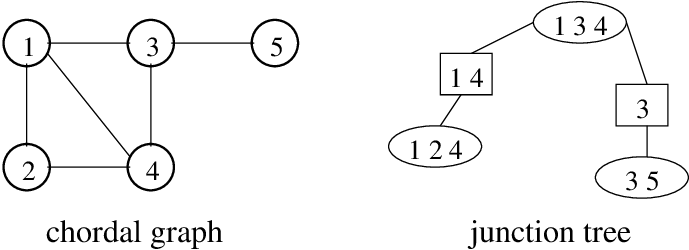
\includegraphics[width=0.98\linewidth]{Pictures/Optimizers/iSAM2/chodar_graph_to_junction_tree_example.png}
    \caption{Picture from Robert Castelo paper \cite{chordal_graph_to_junction_tree_paper} shows an example of a simple Chordal graph (Left side) and corresponding small cliques/junction tree (Right side). Eliminating in a good order produces a chordal Bayes net whose moralized graph can be grouped into cliques/junction trees. This is the structure that keeps $R$ matrix sparse.}
    \label{fig:optimizer-iSAM2-chordal}
\end{figure}
\noindent
When linearizing and eliminating in some order, the resulting triangular system $R$ still satisfies $R^\top R = A^\top A$, but each row block of $R$ matrix now carries a specific meaning. Each row block of $R$ belongs to the variable that was just eliminated. That row says, in Gaussian form, how this variable depends on a few variables that were eliminated earlier. Think of those earlier variables as its parents. When solving $R\Delta\theta=d$ by back substitution, start at the last row and move upward. That is the same as computing each variable from its parents in turn. So $R$ is not just numbers in a triangle. It is the same set of conditional relationships as the Bayes network, written in matrix form.
\\ \\
Because the Bayes net is chordal, its conditionals naturally group into cliques. Consecutive row blocks of $R$ that share the same separator form a clique. Cliques that share a separator are connected to form a Bayes tree. Each clique stores frontal conditionals, child given the parent separator, and each edge carries only the shared separator variables. The tree encodes the same numeric information as $R$, but it is organized by locality rather than by a single global ordering.
\\ \\
\begin{figure}[H]
    \centering
    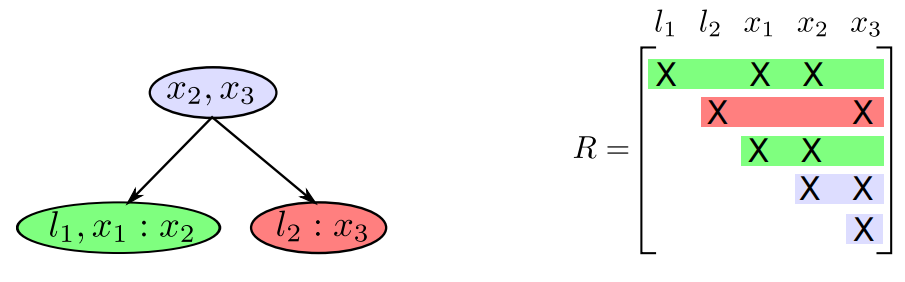
\includegraphics[width=0.98\linewidth]{Pictures/Optimizers/iSAM2/R_matrix_as_bayes_tree1.png}
    \caption{Picture from Bayes tree paper \cite{Bayes_tree_for_SLAM_paper} shows Bayes tree (left) and its matching rows in the square root factor $R$ (right). Colors indicate which contiguous row blocks of $R$ belong to each clique.}
    \label{fig:optimizer-iSAM2-R-to-tree-1}
\end{figure}
\begin{figure}[H]
    \centering
    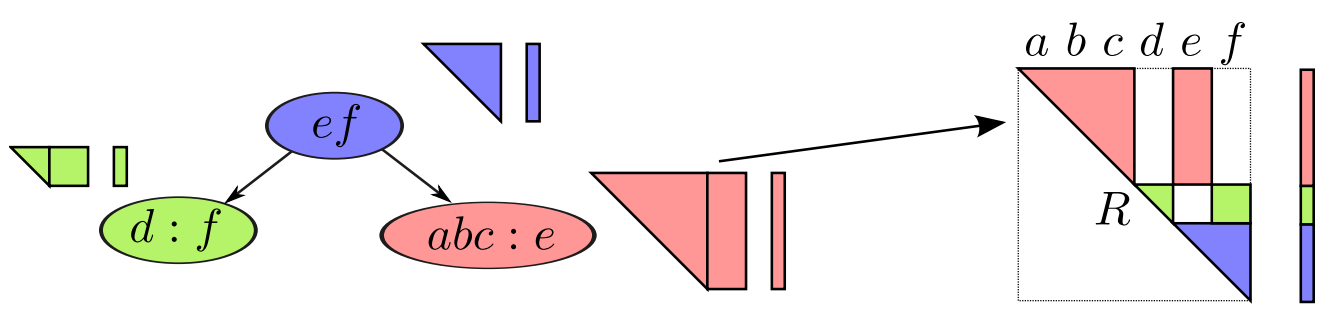
\includegraphics[width=0.98\linewidth]{Pictures/Optimizers/iSAM2/R_matrix_as_bayes_tree2.png}
    \caption{Picture from iSAM2 paper \cite{iSAM2_paper} shows each clique contains the conditional of its frontal variables given the separator. The same entries appear in the corresponding rows/columns of $R$. Back substitution on $R$ mirrors evaluating the tree from leaves to root, while marginal queries follow the few cliques that touch the queried variables.}
    \label{fig:optimizer-iSAM2-R-to-tree-2}
\end{figure}
\noindent
The takeaway is simple. Eliminating a factor graph gives a chordal Bayes net. Grouping its conditionals yields a Bayes tree. The square root factor $R$ contains the very same conditionals in matrix form. Thus $R$ can be viewed as a Bayes tree data structure in matrix form. iSAM2 stores and updates this Bayes tree directly instead of one global $R$, which preserves the numerical benefits of the square root form while enabling strictly local updates. This means when new measurements arrive or when some variables must be re-linearized, only the cliques on a small subtree are touched and the rest of the structure stays unchanged, making computational complexity manageable and the data set grows.



\subsubsection{Incremental Updates directly on Bayes tree}
iSAM2 never rebuilds the whole system when new data arrives. A new odometry or landmark factor only touches a few variables in the factor graph, so only the matching subtree in the Bayes tree is modified. All other branches stay exactly the same. This is the key difference from iSAM, where adding a factor could force a global re-factorization of the single $R$ matrix.
\\ \\
Two simple rules explain why updates stay local. First is that information flows upward in the tree during elimination, so changes propagate only from the touched variables toward the root. Second, a factor becomes active when the first variable in its local elimination order is eliminated, so only the paths from those variables up to the root can be affected, while unrelated subtrees remain untouched.
\\ \\
\begin{figure}[H]
    \centering
    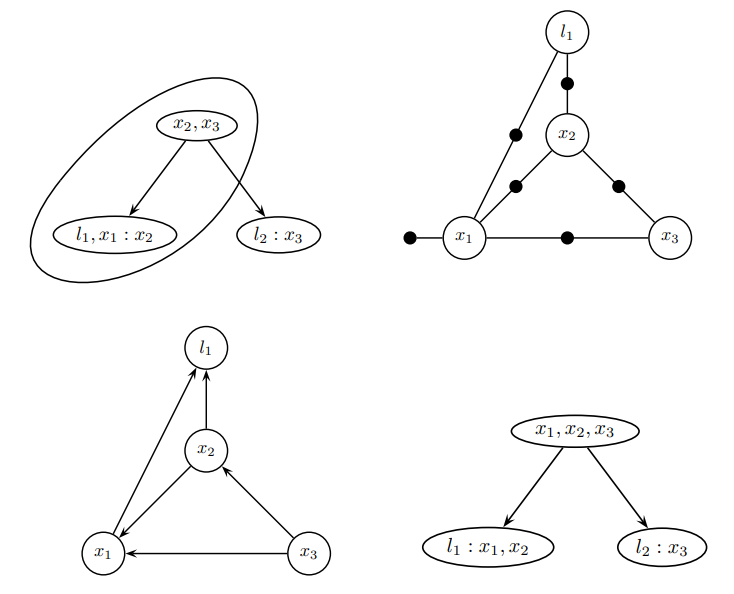
\includegraphics[width=0.98\linewidth]{Pictures/Optimizers/iSAM2/updating_Bayes_tree.png}
    \caption{Picture taken from Bayes tree paper \cite{Bayes_tree_for_SLAM_paper} shows how to update a Bayes tree with a new factor. \\ \noindent 
    (Top left) Affected cliques when adding a factor between $x_1$ and $x_3$, the right branch is unaffected. \\ \noindent
    (Top right) Local factor graph rebuilt from those cliques plus the new factor. \\ \noindent
    (Bottom left) Local chordal Bayes net after elimination. \\ \noindent
    (Bottom right) New Bayes subtree with the untouched ``orphan'' subtree reattached.}
    \label{fig:optimizer-iSAM2-R-update-tree}
\end{figure}
\noindent
One update works as follows. first, locate the cliques that contain the variables touched by the new factor and follow their ancestors up toward the root, this marks the only region that needs work, while the rest of the tree becomes ``orphans'' that stay valid and untouched. Next, convert the conditionals stored in those marked cliques back into a small local factor graph and insert the new factor. Then re-eliminate just this local graph (using the same graph aware elimination as discussed previously) to produce a new chordal Bayes net and its updated Bayes subtree. Finally, reattach the orphan subtrees at the proper separators. Only this small subtree changes, everything else is reused. (See Picture \ref{fig:optimizer-iSAM2-R-update-tree})
\\ \\
The result is incremental and predictable computation. iSAM2 edits only the cliques touched by the new information, runs a small local elimination, and solves by back substitution along that subtree. There are no global re-factorization spikes, and accuracy is maintained by re-linearizing only the variables in the affected region when needed.



\subsubsection{Loop Closure and Incremental Reordering}
\begin{figure}[H]
    \centering
    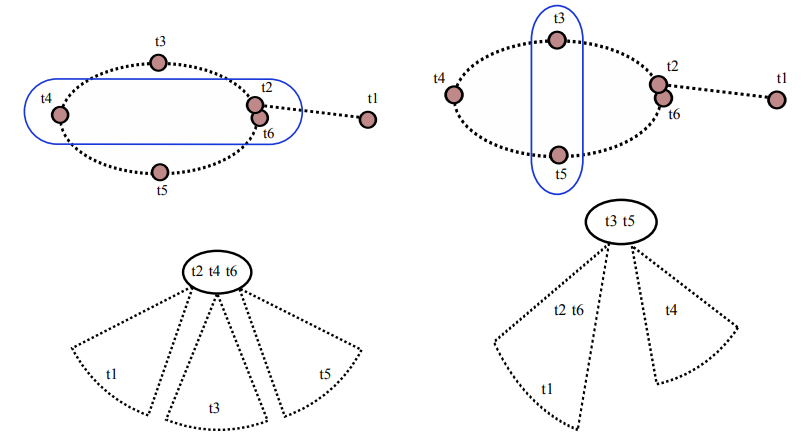
\includegraphics[width=0.98\linewidth]{Pictures/Optimizers/iSAM2/incremental_reordering.png}
    \caption{Picture taken from Bayes tree paper \cite{Bayes_tree_for_SLAM_paper} shows loop closure with incremental reordering. Two batch optimal orderings (top) yield different Bayes trees (bottom). For online operation, the ordering should keep the newest variables near the root, so future updates affect only a small subtree.}
    \label{fig:optimizer-iSAM2-incremental-reordering}
\end{figure}
\noindent
Loop closures add a factor between two far apart poses. In a Bayes tree this never forces a global re-factorization. Only the cliques on the (unique) paths from those two pose cliques up to the root are affected, all other subtrees are untouched ``orphans'' and are reused as is. The affected top region is converted back to a local factor graph, the loop closure factor is added, and the region is re-eliminated to produce a new local chordal Bayes net and Bayes subtree. The unchanged subtrees are then reattached at the matching separators. This keeps updates local and predictable, unlike iSAMs global $R$ re-factorization after loop closure. \cite{iSAM2_paper,Bayes_tree_for_SLAM_paper}
\\ \\
A good variable ordering is still crucial because it controls fill in (clique sizes) during elimination. iSAM2 performs incremental reordering only over the affected variables, rather than periodic global reorderings. A simple and effective rule is to force the most recent variables (the ones new factors usually touch) to be eliminated last (i.e. near the root). Practically, this is implemented with a constrained COLAMD heuristic. Here the newest pose blocks are kept at the end of the order while letting COLAMD algorithm find a sparse order for the rest. This produces small, stable updates at each step, even when loops close. \cite{Bayes_tree_for_SLAM_paper}
\\ \\
Batch orderings found by nested dissection (or similar heuristics) can look equally good for a one time solve because they produce comparable sparsity. For online SLAM the next update matters. The preferred ordering therefore leaves the newest poses at or near the Bayes tree root, so the next odometry or loop closure factor changes only a small subtree. If the newest pose lies deep in the tree, the same update must rewrite many cliques. For this reason iSAM2 uses constrained reorderings, keeping recent variables last in the order near the root and letting the heuristic arrange the rest. This keeps updates local and cheap. \cite{Bayes_tree_for_SLAM_paper}
\\ \\
This constrained COLAMD heuristic will not yield a globally optimal ordering, however it reliably reduces fill in and the amount of work near the update, keeps recent variables near the root, and avoids large latency spikes. In practice it delivers close to batch sparsity while saving compute time, and when needed it is reapplied only to the affected subtree, so the cost stays proportional to that small region rather than the whole tree.



\subsubsection{Fluid Re-Linearization}
iSAM2 stops doing periodic global ``re-linearize everything''. Instead iSAM2 only refresh (re-linearize) the parts of the problem that truly need it, right when they need it. The Bayes tree makes this easy, new measurements change only a small subtree, so iSAM2 recomputes just that piece and leave the rest of the tree alone. This keeps the math accurate without the big stalls that happened in iSAM after loop closures or long runs. \cite{iSAM2_paper,Bayes_tree_for_SLAM_paper}
\\ \\ 
How it works in practice is simple. Always keep a running correction vector $\Delta$ from the latest linear solve. If a variable's change is tiny, treat its current linearization point as ``good enough'' and do not touch it. If a variable's change is larger than a small threshold (call it $\beta$), mark that variable for re-linearization. Then mark the cliques that contain those variables and their ancestors in the Bayes tree. Only those cliques are rebuilt, go back to the original nonlinear factors for those cliques, recompute their Jacobians at the new linearization point, add cached ``marginal'' factors from untouched children, and eliminate again to update just the top of the tree. Everything else remains as it was. Note that this re-linearization threshold can be set per state. Positions $(x,y)$ can use a looser (higher) threshold so they are refreshed less often, while the heading angle, being more nonlinear should use a tighter (lower) threshold. \cite{Bayes_tree_for_SLAM_paper}
\\ \\
Solving for $\Delta\theta$ is also done only where needed. First solve on the modified top of the tree. Then walk into children only if any parent update exceeded a small propagation threshold (call it $\alpha$). This ``only follow when it matters'' rule avoid needless work in distant parts of the map while still keeping accuracy where the robot is and where measurements arrived. Together, the two thresholds ($\beta$ to decide who to re-linearize, and $\alpha$ to decide where to propagate the solve) give iSAM2 its fluid, real-time/online behavior. Accuracy when and where it matters, speed everywhere else.
\\ \\
This local, threshold strategy removes the need for heavy batch steps and keeps runtime smooth over long missions just like incremental reordering does the same. In essence what iSAM2 does is it exploits Factor graphs representations of the map and Bayes tree data structure to do dynamic variable reordering and re-linearization, no need for periodic batch calculations like in iSAM. On standard datasets (Victoria Park) the cumulative computation of iSAM2 grows much more slowly than iSAM, because re-linearization and re-elimination are confined to small subtrees rather than the full graph. And over time the discrepancy will only grow where iSAM will slow down whilst iSAM2 will hold its compute much more efficient. (See Picture \ref{fig:optimizer-iSAM2-fluid-relin})
\\ \\
\begin{figure}[H]
  \centering
  \begin{minipage}[t]{0.35\linewidth}
    \centering
    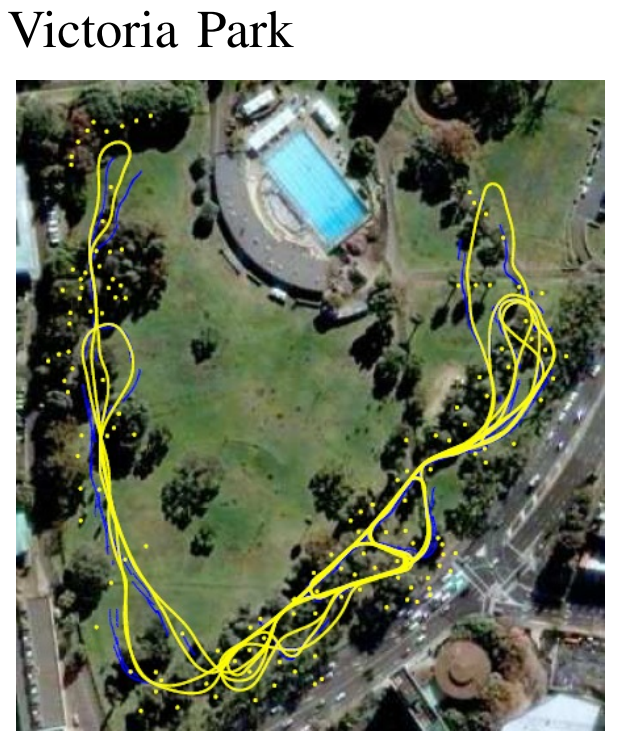
\includegraphics[width=\linewidth]{Pictures/Optimizers/iSAM2/Victoria_park_map.png}
    \caption*{\small Victoria Park SLAM map used in the original iSAM benchmarks.}
  \end{minipage}\hfill
  \begin{minipage}[t]{0.55\linewidth}
    \centering
    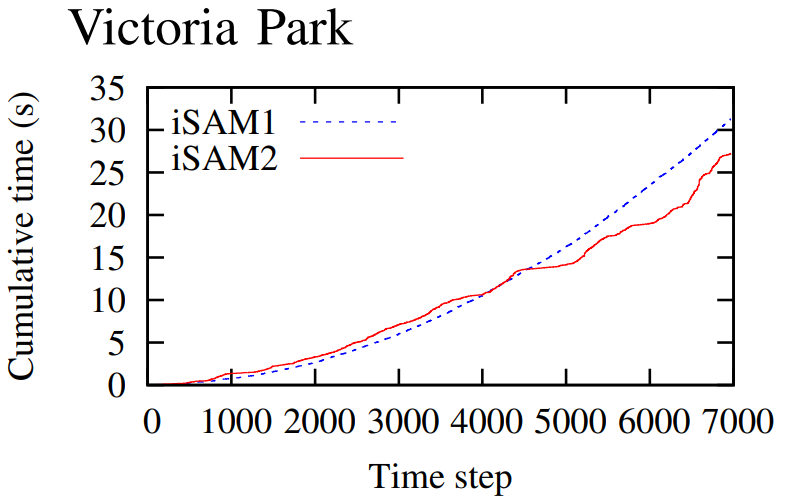
\includegraphics[width=\linewidth]{Pictures/Optimizers/iSAM2/Victoria_park_graph.png}
    \caption*{\small Cumulative time vs. step for iSAM (periodic batch) and iSAM2 (fluid). iSAM2 stays faster as the dataset grows.}
  \end{minipage}
  \caption{Picture from the Bayes tree paper \cite{Bayes_tree_for_SLAM_paper}. In iSAM2, relinearization is fluid, only the affected cliques are recomputed and the rest of the tree is reused.}
  \label{fig:optimizer-iSAM2-fluid-relin}
\end{figure}



\subsubsection{Sparse Factor Graphs}
Over long missions the factor graph can accumulate many near duplicate constraints (revisits of the same place, repeated landmark sightings from similar viewpoints). This “Eiffel Tower effect” slowly densifies the graph and enlarges cliques in the Bayes tree, which increases update cost. The fix is sparsification. Here keep the informative constraints and summarize or drop the redundant data points while preserving the important information flow. In practice this is done locally where data arrive. Retain the freshest odometry and a few diverse loop closures, and replace discarded constraints by a light summary on the small separator set where they would have entered the tree. Intuitively, keep the ``shape'' of the information at the boundary and forget interior details that are now redundant. Simple policies such as keyframing (keeping only selected poses as variables), pruning highly correlated measurements, and limiting per landmark observation count work well. The result is a graph that stays sparse, cliques that stay small, and a Bayes tree that remains cheap to update even in very long runs.



\subsubsection{Beyond Gaussian Assumptions (Robust Estimators)}
Pure Gaussian residuals are fragile in the face of outliers (bad data association, spurious loop closures, moving objects, changing environment). Robust estimators fix this by replacing the quadratic loss with a robust loss that grows slower than a square. Common choices include Huber (quadratic near zero, linear in the tails), Cauchy, or Tukey. In iSAM2 this is a drop in change at the factor level. Each robust loss yields a weight for its residual, updated as the estimate improves (iteratively re-weighted least squares). Factors that fit well keep high weight, inconsistent ones are down weighted, so they no longer dominate the solution. This makes incremental updates and fluid re-linearization safer because a single wrong constraint will not trigger large edits high up in the tree. For hard loop closures, one can also use switchable or graduated penalties that let the optimizer ``turn off'' a suspect factor until there is enough supporting evidence. The Bayes tree concept stays the same, only local factor weights and linearization adapt, so robustness comes with little extra complexity.



\subsubsection{Data Association from the Bayes Tree}
The same as in iSAM, iSAM2 scores candidate matches with a Mahalanobis distance, which measures the innovation in units of its uncertainty. However in iSAM2 the needed covariances are read directly from the Bayes tree without forming a dense matrix. Pose and nearby pose to landmark covariances are obtained efficiently by following only the few cliques that contain those variables and their separators. This keeps online/real-time gating fast for data association. Queries involving far away landmarks or many old poses may touch a larger portion of the tree and therefore cost more, but they remain practical on demand. In practice this combines a cheap, conservative bound (for routine gating) with exact small block queries when decisions are critical (eks verifying a loop closure). The result is reliable association with predictable compute cost during operation.



\subsubsection{Algorithm}
At each step iSAM2 absorbs new measurements, touch only the relevant cliques in the Bayes tree, solve for a small increment, and update the state. iSAM2 combines the linear update with fluid re-linearization, so work stays local and predictable. Concretely, one iteration looks like this (matching the structure summarized in the iSAM2 and Bayes tree papers \cite{iSAM2_paper,Bayes_tree_for_SLAM_paper})
\begin{enumerate}
    \item \textbf{Add new data:} Insert the new factors (odometry, measurements, loop closures) into the factor graph. If new states appear, add them to the estimate $\Theta$.

    \item \textbf{Mark what to refresh (fluid re-linearization):} Keep the last increment $\Delta\theta$. If a state moved more than a small threshold $\beta$, mark it for re-linearization. Only pass this mark to neighbors if the parent changed more than a smaller threshold $\alpha$. This finds the small set that really needs work now.

    \item \textbf{Build a small local problem:} Take just the cliques in the Bayes tree that touch the marked states (and their ancestors up to the root) and turn them back into a tiny factor graph, everything else becomes reusable ``orphans''.

    \item \textbf{Order and eliminate locally:} Find a sparse order for this small graph using a constrained COLAMD (keep the newest states last, near the root), then eliminate to make a new local Bayes subtree.

    \item \textbf{Reattach orphans:} Connect the untouched subtrees back at the correct separators. Only the edited subtree changed, the rest is reused.

    \item \textbf{Solve where needed:} Back solve on the updated top of the tree to get a new increment $\Delta\theta$. Propagate the solve into children only when the parent's change is big enough (same $\alpha$ rule).

    \item \textbf{Update the estimate:} Apply the increment on the whole factor graph, $\Theta \leftarrow \Theta \oplus \Delta\Theta$ (where $\theta = \Theta$ and $\Delta\theta = \Delta\Theta$). Keep $\Delta\Theta$ for the next steps re-linearization test.

    \item \textbf{Keep variable ordering healthy (incremental):} When a loop closure grows cliques near the root, run constrained COLAMD again, but only on that small region to reduce fill and keep the newest states near the root.
    
    \item \textbf{Data association update:} Fetch the needed local covariances from the Bayes tree, compute far away covariances only on demand, and compare predicted and observed features using chosen Data Association method.
\end{enumerate}



\subsubsection{Limitations}
While iSAM2 removes the big computation spikes seen in iSAM, some practical and theoretical limits remain.

\begin{itemize}
  \item \textbf{Ordering is heuristic, not optimal:} Choosing a variable order that minimizes fill in is NP-hard, so iSAM2 relies on constrained COLAMD and related heuristics. These give good, stable performance online but cannot guarantee the globally best sparsity.

  \item \textbf{Clique growth in dense areas.} Heavy revisiting of the same places (``Eiffel Tower effect'') or many near duplicate constraints can enlarge cliques near the root. Updates remain local, but the cost of each local elimination grows with clique size. In long runs, sparsification/keyframing is often needed to keep the graph light.

  \item \textbf{Threshold tuning for fluid re-linearization:} The accuracy/speed trade off depends on two small thresholds (who to re-linearize and how far to propagate the solve). These must be tuned for the sensor and motion model. Too loose can delay accuracy, too tight does extra work.

  \item \textbf{Faraway covariances can be expensive:} Exact marginal/covariance queries are done by recursive message passing on the tree (dynamic programming style). Queries that span long paths or large separators touch more cliques and therefore cost more.

  \item \textbf{Gaussian least-squares core:} Outliers and non Gaussian effects are not handled by iSAM2 alone. Robust losses or switchable constraints must be added at the factor level to down weight bad data, otherwise accuracy can degrade during long missions.

  \item \textbf{Nonlinearity still matters:} Poor initial guesses or highly nonlinear measurements can require multiple Gauss-Newton/Levenberg-Marquardt steps. iSAM2 just makes each step local.

  \item \textbf{Engineering complexity and memory:} Compared to a single global $R$ in iSAM, the Bayes tree in iSAM2 adds much more moving parts (cliques, separators, cached/orphan subtrees, incremental reordering). Correct, efficient implementations are more involved, and memory still grows with map size unless one prunes or summarizes.
\end{itemize}
\noindent 
In practice, most of these limits can be mitigated with careful design. Using keyframing/sparsification to cap clique size, robust losses or switchable constraints to handle outliers, and constrained incremental reordering to keep updates local. The main hurdle is engineering complexity. This is where the open source \textbf{GTSAM} library (from the Georgia Tech team behind iSAM/iSAM2) is invaluable. It ships a production quality Bayes tree/iSAM2 implementation, clean factor graph APIs, robust noise models, and utilities for ordering and re-linearization, making it a practical starting point for both research and deployment.

